\chapter{Конструкторская часть}

\section{Описание сущностей базы данных и их связей}\label{sec:сущности}

Согласно ER-диаграмме сущностей в нотации Чена в проектируемой базе данных были выделены 9 таблиц для сущностей, которые уже определены в аналитической части, и 1 дополнительная таблица для реализации связи <<многие ко многим>> между клиентами и товарами.
На рисунке~\ref{fig:diag} изображена диаграмма проектируемой базы данных.

Рассмотрим подробнее каждую таблицу и ее поля.

Таблица пользователей, содержащая информацию о пользователях фитнес-клуба, содержит поля, описанные в таблице~\ref{tbl:pol_user}.
\begin{table}[h!]
	\begin{center}
		\begin{threeparttable}
			\captionsetup{justification=raggedright,singlelinecheck=off}
			\caption{\label{tbl:pol_user} Поля таблицы пользователей}
			\begin{tabular}{|p{4cm}|p{4cm}|p{6cm}|}
				\hline
				Поле & Тип & Описание \\
				\hline
				id\_user & целое & Идентификатор пользователя \\
				\hline
				role & строка & Роль пользователя (клиент, тренер, администратор) \\
				\hline
				email & строка & email пользователя \\
				\hline
				password & строка & Пароль пользователя \\
				\hline
			\end{tabular}
		\end{threeparttable}
	\end{center}
\end{table}

Таблица тренеров, содержащая информацию о тренерах фитнес-клуба, содержит поля, описанные в таблице~\ref{tbl:pol_trainers}.
\begin{table}[h!]
	\begin{center}
		\begin{threeparttable}
			\captionsetup{justification=raggedright,singlelinecheck=off}
			\caption{\label{tbl:pol_trainers} Поля таблицы тренеров}
			\begin{tabular}{|p{4cm}|p{4cm}|p{6cm}|}
				\hline
				Поле & Тип & Описание \\
				\hline
				id\_trainer & целое & Идентификатор тренера \\
				\hline
				id\_user & целое & Идентификатор пользователя \\
				\hline
				name & строка & ФИО тренера \\
				\hline
				gender & строка & Пол тренера \\
				\hline
				specialization & строка & Специализация тренера \\
				\hline
				experience & целое & Стаж тренера \\
				\hline
				rating & целое & Рейтинг тренера \\
				\hline
			\end{tabular}
		\end{threeparttable}
	\end{center}
\end{table}

Таблица администраторов, содержащая информацию об администраторах фитнес-клуба, содержит поля, описанные в таблице~\ref{tbl:pol_admins}.
\begin{table}[h!]
	\begin{center}
		\begin{threeparttable}
			\captionsetup{justification=raggedright,singlelinecheck=off}
			\caption{\label{tbl:pol_admins} Поля таблицы администраторов}
			\begin{tabular}{|p{4cm}|p{4cm}|p{6cm}|}
				\hline
				Поле & Тип & Описание \\
				\hline
				id\_admin & целое & Идентификатор администратора \\
				\hline
				id\_user & целое & Идентификатор пользователя \\
				\hline
				name & строка & ФИО администратора \\
				\hline
				data\_of\_birth & дата & Дата рождения администратора \\
				\hline
				gender & строка & Пол администратора \\
				\hline
			\end{tabular}
		\end{threeparttable}
	\end{center}
\end{table}

Таблица клиентов, содержащая информацию о клиентах фитнес-клуба, содержит поля, описанные в таблице~\ref{tbl:pol_clients}.
\begin{table}[h!]
	\begin{center}
		\begin{threeparttable}
			\captionsetup{justification=raggedright,singlelinecheck=off}
			\caption{\label{tbl:pol_clients} Поля таблицы клиентов}
			\begin{tabular}{|p{4cm}|p{4cm}|p{6cm}|}
				\hline
				Поле & Тип & Описание \\
				\hline
				id\_client & целое & Идентификатор клиента \\
				\hline
				id\_user & целое & Идентификатор пользователя \\
				\hline
				name & строка & ФИО клиента \\
				\hline
				gender & строка & Пол клиента \\
				\hline
				data\_of\_birth & дата & Дата рождения клиента \\
				\hline
				id\_membership & целое & Идентификатор абонемента \\
				\hline
				membership\_end & дата & Дата окончания абонемента \\
				\hline
			\end{tabular}
		\end{threeparttable}
	\end{center}
\end{table}

Таблица бонусов, содержащая информацию о бонусах клиентов фитнес-клуба, содержит поля, описанные в таблице~\ref{tbl:pol_bonus}.
\begin{table}[h!]
\begin{center}
	\begin{threeparttable}
		\captionsetup{justification=raggedright,singlelinecheck=off}
		\caption{\label{tbl:pol_bonus} Поля таблицы бонусов}
		\begin{tabular}{|p{4cm}|p{4cm}|p{6cm}|}
			\hline
			Поле & Тип & Описание \\
			\hline
			id\_bonus & целое & Идентификатор записи о бонусах \\
			\hline
			id\_client & целое & Идентификатор клиента \\
			\hline
			count & целое & Количество бонусов \\
			\hline
		\end{tabular}
	\end{threeparttable}
\end{center}
\end{table}


Таблица абонементов, содержащая информацию об абонементах фитнес-клуба, содержит поля, описанные в таблице~\ref{tbl:pol_mem}.
\begin{table}[h!]
	\begin{center}
		\begin{threeparttable}
			\captionsetup{justification=raggedright,singlelinecheck=off}
			\caption{\label{tbl:pol_mem} Поля таблицы абонементов}
			\begin{tabular}{|p{4cm}|p{4cm}|p{6cm}|}
				\hline
				Поле & Тип & Описание \\
				\hline
				id\_membership & целое & Идентификатор абонемента \\
				\hline
				name & строка & Название абонемента \\
				\hline
				duration & промежуток времени & Длительность абонемента \\
				\hline
				price & целое & Цена абонемента \\
				\hline
				freezing & целое & Длительность возможной заморозки абонемента \\
				\hline
			\end{tabular}
		\end{threeparttable}
	\end{center}
\end{table}

Таблица тренировок, содержащая информацию о тренировках, которые проводятся в фитнес-клубе, содержит поля, описанные в таблице~\ref{tbl:pol_work}.
\begin{table}[h!]
	\begin{center}
		\begin{threeparttable}
			\captionsetup{justification=raggedright,singlelinecheck=off}
			\caption{\label{tbl:pol_work} Поля таблицы тренировок}
			\begin{tabular}{|p{4cm}|p{4cm}|p{6cm}|}
				\hline
				Поле & Тип & Описание \\
				\hline
				id\_workout & целое & Идентификатор тренировки \\
				\hline
				name & строка & Название тренировки \\
				\hline
				description & строка & Описание тренировки \\
				\hline
				id\_trainer & целое & Идентификатор тренера \\
				\hline
				duration & промежуток времени & Длительность тренировки \\
				\hline
				level & целое & Сложность тренировки (от 1 до 5) \\
				\hline
			\end{tabular}
		\end{threeparttable}
	\end{center}
\end{table}

Таблица расписания, содержащая информацию о расписании фитнес-
клуба, содержит поля, описанные в таблице~\ref{tbl:pol_shed}.
\begin{table}[h!]
	\begin{center}
		\begin{threeparttable}
			\captionsetup{justification=raggedright,singlelinecheck=off}
			\caption{\label{tbl:pol_shed} Поля таблицы расписания}
			\begin{tabular}{|p{4cm}|p{4cm}|p{6cm}|}
				\hline
				Поле & Тип & Описание \\
				\hline
				id\_record & целое & Идентификатор записи \\
				\hline
				id\_workout & целое & Идентификатор тренировки \\
				\hline
				data\_and\_time & дата и время & Дата и время тренировки \\
				\hline
				id\_client & целое & Идентификатор клиента (NULL, если групповая) \\
				\hline
			\end{tabular}
		\end{threeparttable}
	\end{center}
\end{table}

Таблица товаров, содержащая информацию о услугах и товарах фитнес-клуба, содержит поля, описанные в таблице~\ref{tbl:pol_good}.
\begin{table}[h!]
	\begin{center}
		\begin{threeparttable}
			\captionsetup{justification=raggedright,singlelinecheck=off}
			\caption{\label{tbl:pol_good} Поля таблицы товаров}
			\begin{tabular}{|p{4cm}|p{4cm}|p{6cm}|}
				\hline
				Поле & Тип & Описание \\
				\hline
				id\_good & целое & Идентификатор товара/услуги \\
				\hline
				name & строка & Название товара/услуги \\
				\hline
				price & целое & Цена товара/услуги \\
				\hline
			\end{tabular}
		\end{threeparttable}
	\end{center}
\end{table}

Таблица, связывающая клиентов и товары, которые они приобрели, содержит поля, описанные в таблице~\ref{tbl:pol_client_good}.
\begin{table}[h!]
	\begin{center}
		\begin{threeparttable}
			\captionsetup{justification=raggedright,singlelinecheck=off}
			\caption{\label{tbl:pol_client_good} Поля таблицы, связывающей клиентов и приобретенные ими товары}
			\begin{tabular}{|p{4cm}|p{4cm}|p{6cm}|}
				\hline
				Поле & Тип & Описание \\
				\hline
				id & целое & Идентификатор записи о покупке \\
				\hline
				id\_client & целое & Идентификатор клиента \\
				\hline
				id\_good & целое & Идентификатор товара/услуги \\
				\hline
			\end{tabular}
		\end{threeparttable}
	\end{center}
\end{table}

\clearpage

\begin{figure}[h!]
	\centering
	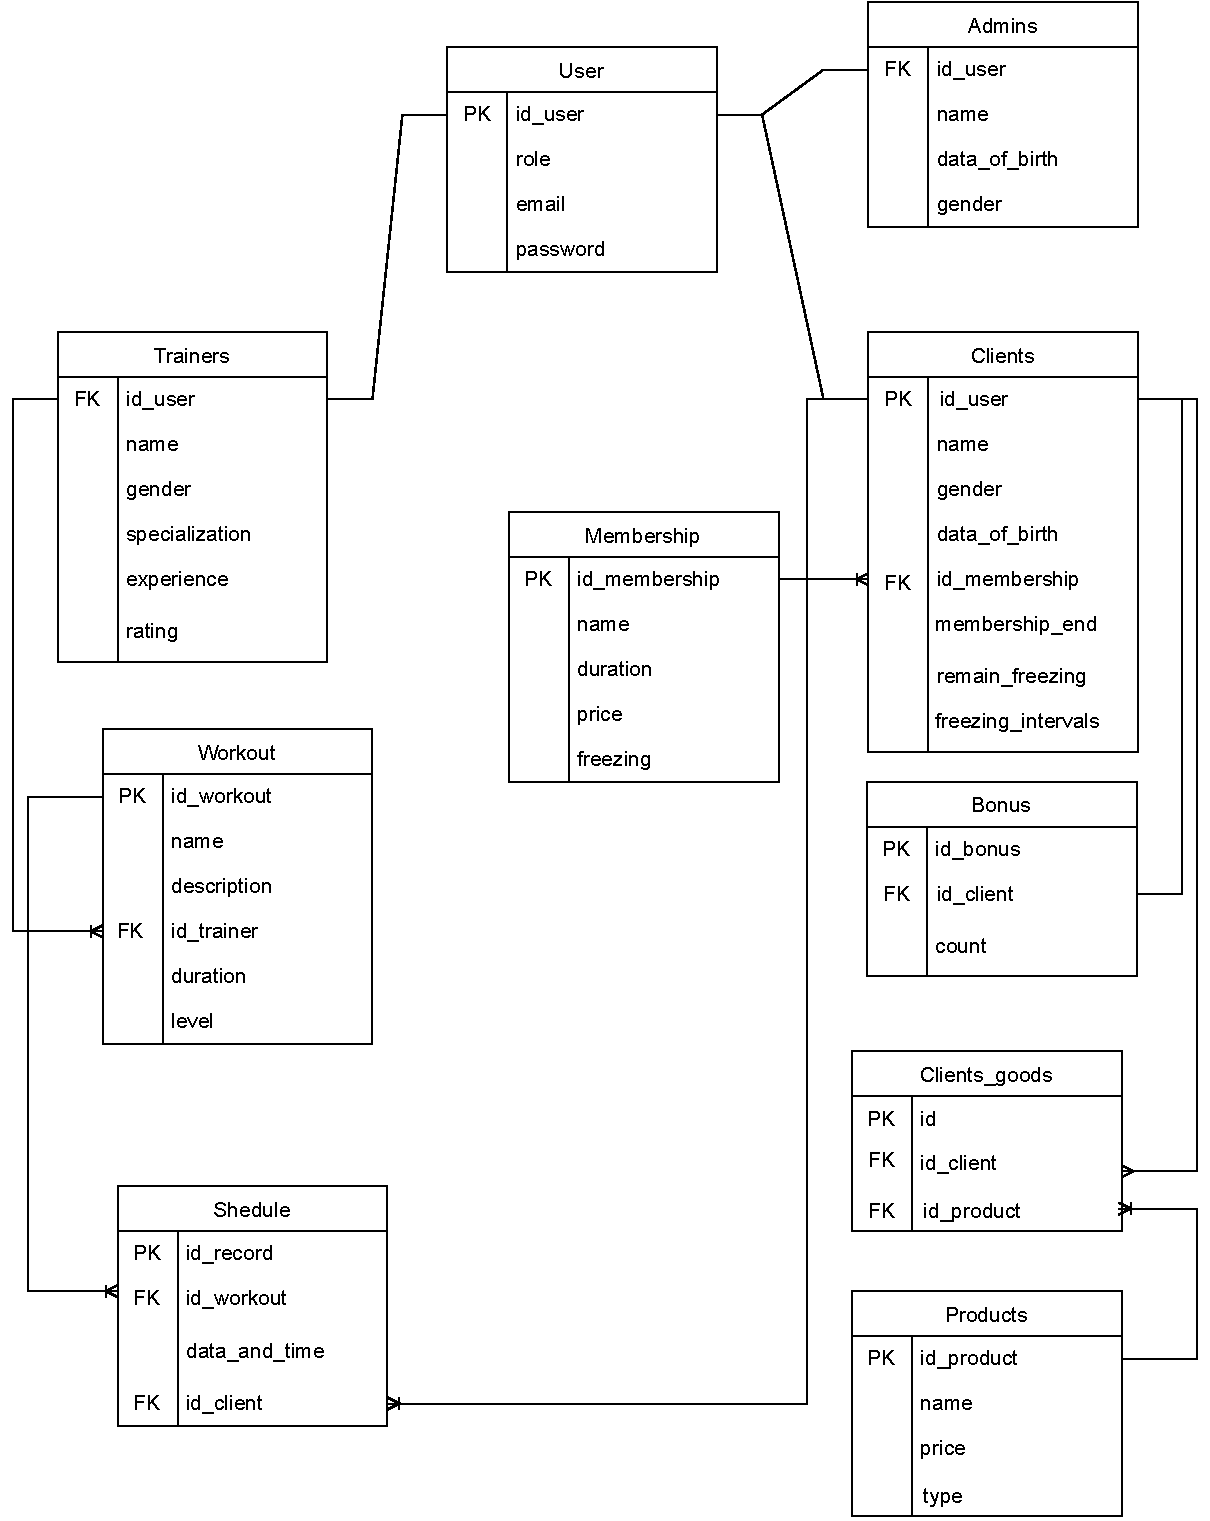
\includegraphics[width=\linewidth]{img/diagramma}
	\caption{Диаграмма проектируемой базы данных}
	\label{fig:diag}
\end{figure}

\section{Роли базы данных}\label{sec:роли}
На основе пунктов работы \ref{sec:предмет}, \ref{sec:формализация} и \ref{sec:сущности} были определены следующие роли и их права доступа в проектируемой базы данных.

\begin{enumerate}[label=\arabic*)]
	\item Гость: возможность просмотра данных таблиц Membership, Goods, Workout, Shedule и Trainers.
	\item Клиент: возможность просмотра данных таблиц Membership, Goods, \newline Workout, Shedule и Trainers, своей строки в таблице Bonus, а также добавлять записи в таблицу Shedule (с помощью записи на персональную тренировку).
	\item Тренер: возможность просмотра данных таблиц Membership, Goods, \newline Workout, Shedule Trainers и Clients, а также добавлять записи в таблицу Shedule (с помощью добавления персональных и групповых тренировок) и в таблицу Workout (с помощью создания новых тренировок).
	\item Администратор: возможность просматривать и изменять все таблицы.
\end{enumerate}

\section{Триггер базы данных}\label{sec:триггер}

При желании клиента купить товар важно правильно рассчитать количество бонусов, которое спишется и начислится, а так же нужно, чтобы при каждой покупке товара они сразу начислялись, иначе может произойти ситуация, что товар будет куплен, а бонусы не списаны.

Поэтому при каждой покупке товара должна вызываться функция, схема которой изображена на рисунке~\ref{fig:trigger}.
\clearpage
\begin{figure}[h!]
	\centering
	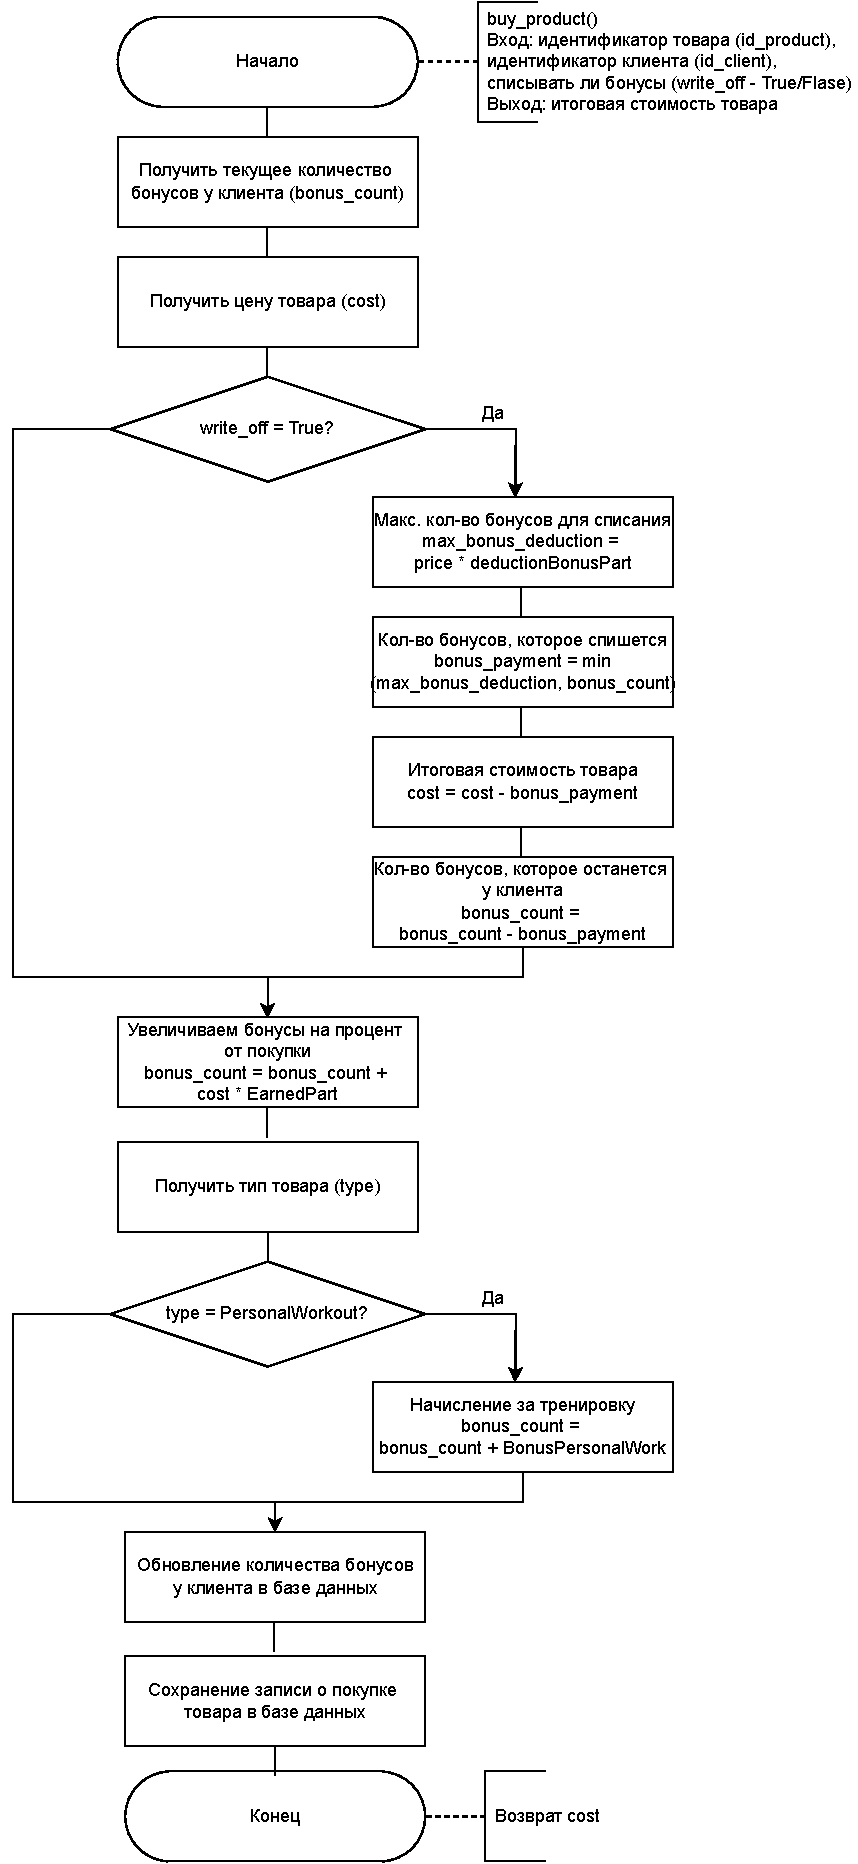
\includegraphics[width=0.65\linewidth]{img/trigger}
	\caption{Схема алгоритма вычисления итоговой стоимости и обновлении бонусов}
	\label{fig:trigger}
\end{figure}
\clearpage


\section*{Выводы к конструкторской части}

В этой части работы были описаны сущности проектируемой базы данных, а также ее роли и трииггер.